\documentclass[12pt]{exam}
\usepackage[top=1in, bottom=1in, left=.45in, right=.45in]{geometry}
\usepackage{amsmath,amsthm,amssymb,amstext}
\usepackage{enumerate,enumitem}
\usepackage{tikz,float,graphicx}
\usepackage{microtype}
\usepackage{multicol}
\usepackage{bm}
\usepackage[framemethod=tikz]{mdframed}

\newcommand{\course}{MTH 234 Summer 2021}
\newcommand{\qdate}{Vectors} %PUT DATE HERE
\newcommand{\quiz}{Group Work} 
\newcommand{\gen}[1]{\left\langle #1 \right\rangle}
\newcommand{\ba}{\bm{a}}
\newcommand{\bb}{\bm{b}}
\newcommand{\bc}{\bm{c}}

\newtheorem*{definition}{Definition}
\surroundwithmdframed[]{definition}
\newtheorem*{theorem}{Theorem}
\surroundwithmdframed[]{theorem}

%%%%%%%%%%%%%%%%%%%%%%%
% HEADER AND FOOTER
%%%%%%%%%%%%%%%%%%%%%%%
\pagestyle{headandfoot}
\firstpageheadrule
\runningheadrule
\firstpageheader{\course}{\quiz}{\qdate}
\runningheader{\course}{\quiz}{\qdate}
\runningfooter{}{}{}


\usepackage{color}
\shadedsolutions
\definecolor{SolutionColor}{rgb}{0.8,0.9,1}
\printanswers
%\noprintanswers


\begin{document}
\section*{Vector Operations Learning Objectives}
  \begin{itemize}
    \item{
      Define vector addition and scalar multiplication.
    }
    \item{
      Deduce some properties of vector addition and scalar multiplication.
    }
  \end{itemize}
  
\section*{Vector Operations Examples}
  \begin{definition}
    Let $\mathbf{a}=\langle a_{1},a_{2},a_{3}\rangle$ and $\mathbf{b}=\langle b_{1},b_{2},b_{3}\rangle$ be position vectors and $c$ a scalar (i.e. $c$ is a real number).
    We define
    \begin{gather*}
      \mathbf{a}+\mathbf{b}=\langle a_{1}+b_{1},a_{2}+b_{2},a_{3}+b_{3}\rangle \\
      c\mathbf{a}=\langle ca_{1},ca_{2},ca_{3}\rangle.
    \end{gather*}
    Vector addition and scalar multiplication is defined similarly for position vectors in the plane.
    \end{definition}
    
\begin{enumerate}
    \item{Consider the vectors $\mathbf{a}=\langle 1,3\rangle$ and $\mathbf{b}=\langle -3,2\rangle$.
        \begin{enumerate}
        \item{
                Evaluate $\mathbf{a}+\mathbf{b}$.
                \begin{solution}
                \[
                    \gen{1,3}+\gen{-3,2}=\gen{1-3,3+2}=\gen{-2,5}
                \]
                \end{solution}
            }
        \item{
           On a single graph, draw the position vectors $\mathbf{a}$, $\mathbf{b}$, and $\mathbf{a}+\mathbf{b}$.
           On the same graph, draw the vector equal to $\mathbf{b}$ with initial point $(1,3)$.
           Similarly, draw the vector equal to $\mathbf{a}$ with initial point $(-3,2)$.
           Briefly explain why vector addition is called the parallelogram law.}
        \begin{solution}
            The vectors form a parallelogram when positioned this way.
            \begin{center}
                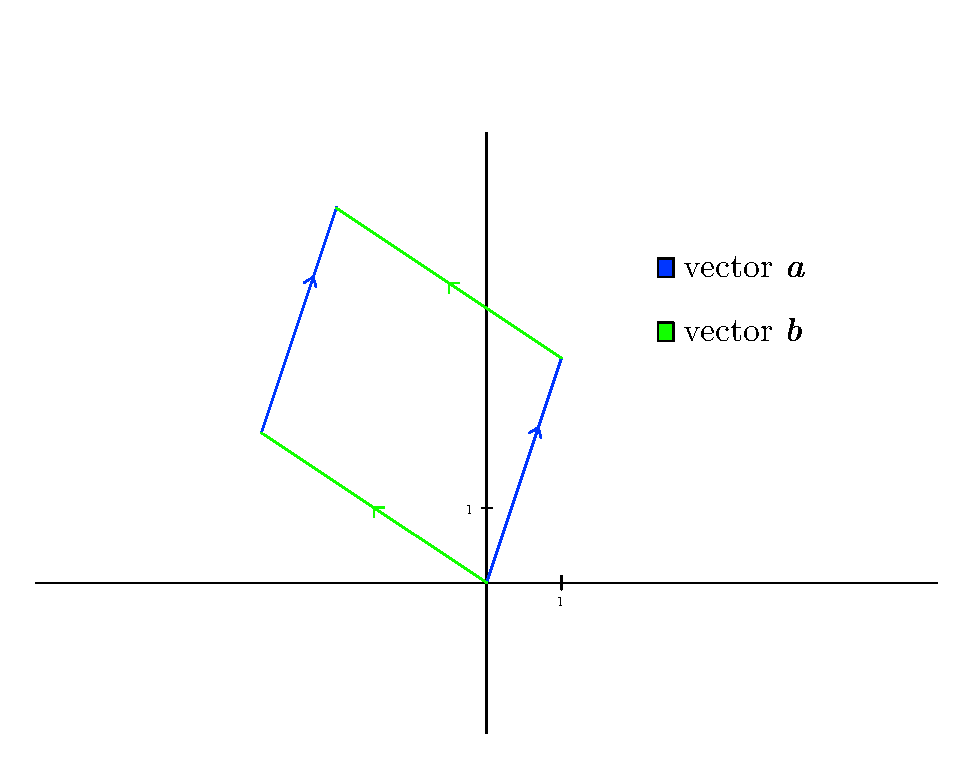
\includegraphics[width=.55\textwidth]{12-1-paral.pdf}
            \end{center}
        \end{solution}
         \item{Evaluate $2\mathbf{a}$ and $-\mathbf{a}$.}

            \begin{solution}
                \[
                2\ba = \gen{2,6}
                \]
                \[
                    -\ba = \gen{-1,-3}
                \]
            \end{solution}
         
         \item{On a single graph, draw the position vectors $\mathbf{a}$, $2\mathbf{a}$, and $-\mathbf{a}$. Explain why $c\mathbf{a}$ is called scalar multiplication.
         }

            \begin{solution}
                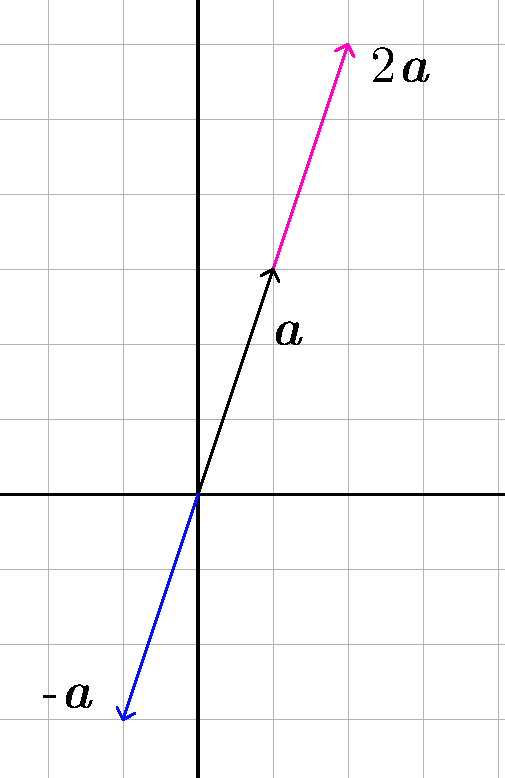
\includegraphics[width=.25\textwidth]{12-2-vectorsa2a.pdf}
            \end{solution}

         \item{
           Evaluate $-3\mathbf{a}+2\mathbf{b}$.
           
           Vector addition and scalar multiplication follows the ``usual" order of operations.
           Namely, $-3\mathbf{a}+2\mathbf{b}=(-3\mathbf{a})+(2\mathbf{b})$.
         }

            \begin{solution}
            \begin{align*}
                -3\ba+2\bb & = -3\gen{1,3}+2\gen{-3,2}\\
                & = \gen{-3,-9}+\gen{-6,4}\\
                & = \gen{-9,-5}
            \end{align*}
            \end{solution}
       
       \end{enumerate} 
    }
  \end{enumerate}
  
  \begin{theorem}
    If $\mathbf{a}$ is a position vector and $c$ is a scalar then $||c\mathbf{a}||=|c||\cdot||\mathbf{a}||$.
  \end{theorem}
  
  \begin{enumerate}
    \item[2.]{
      \begin{enumerate}
        \item{
          Consider $c=-10$ and $\mathbf{a}=\langle 1,3,0\rangle$.
          Evaluate both $||c\mathbf{a}||$ and $|c|\cdot||\mathbf{a}||$ to show that the theorem holds in this case.
        }
            \begin{solution}
                \begin{align*}
                    ||c\ba|| & = ||-10\gen{1,3,0}||\\
                        & = ||\gen{-10,-30,0}||\\
                        & = \sqrt{(-10)^2+(-30)^2+0^2}\\
                        & = \sqrt{100+900}\\
                        & = \sqrt{1000} = 10\sqrt{10}.
                \end{align*}
and
                \begin{align*}
                    |c| ||\ba|| & = |-10| ||\gen{1,3,0}||\\
                    & = 10\sqrt{1^2+3^2+0^2}\\
                    & = 10\sqrt{10}.
                \end{align*}
            \end{solution}
        \item{
          Prove the above theorem.
          
          \textit{Hint:}
          Write $\mathbf{a}=\langle a_{1},a_{2},a_{3}\rangle$, expand $||c\mathbf{a}||$, then factor out $\sqrt{c^{2}}$.
        }
            \begin{solution}
            \begin{align*}
                ||c\ba|| & = ||c\gen{a_1,a_2,a_3}||\\
                    & = ||\gen{ca_1,ca_2,ca_3}||\\
                    & = \sqrt{(ca_1)^2+(ca_2)^2+(ca_3)^2}\\
                    & = \sqrt{c^2a_1^2+c^2a_2^2+c^2a_3^2}\\
                    & = \sqrt{(c^2)(a_1^2+a_2^2+a_3^2)}\\
                    & = \sqrt{c^2}\sqrt{a_1^2+a_2^2+a_3^2}\\
                    & = |c| ||\ba||
            \end{align*}
            \end{solution}
      


      \end{enumerate}
    }
  \end{enumerate}
  
  \begin{definition}
    We say that a vector $\mathbf{a}$ is a \textbf{unit vector} if $||\mathbf{a}||=1$.
  \end{definition}

  \begin{enumerate}
    \item[3.]{
      \begin{enumerate}
        \item{
          Find a unit vector in the same direction as $\mathbf{a}=\langle 1,2,3\rangle$.
      
          \textit{Hint:}
          Apply the above theorem with $c=1/||\mathbf{a}||$.
        }

            \begin{solution}
            \[
                \dfrac{1}{|\ba|}\ba = \dfrac{1}{\sqrt{14}}\gen{1,2,3} = \gen{\dfrac{1}{\sqrt{14}},\dfrac{2}{\sqrt{14}},\dfrac{3}{\sqrt{14}}}
            \]
            \end{solution}
        
        \item{
          Find a vector of length $3$ in the direction opposite of $\mathbf{a}=\langle -2,4,1\rangle$.
          
          \textit{Hint:}
          How is opposite direction related to scalar multiplication.
          Look at Problem 1d above.
        }

            \begin{solution}
                Length 3:
                \[
                    3\left(\frac{\ba}{|\ba|}\right) = \gen{\dfrac{3}{\sqrt{14}},\dfrac{6}{\sqrt{14}},\dfrac{9}{\sqrt{14}}}
                \]
                Opposite direction:
                \[
                    -1\left(\frac{\ba}{|\ba|}\right) = \gen{-\dfrac{1}{\sqrt{14}},-\dfrac{2}{\sqrt{14}},-\dfrac{3}{\sqrt{14}}}
                \]
            \end{solution}
      \end{enumerate}
    }
  \end{enumerate}
  




  \begin{theorem}
    If $\mathbf{a}\neq\langle 0,0,0\rangle$ then $\mathbf{a}/||\mathbf{a}||$ is a unit vector in the same direction as $\mathbf{a}$.
  \end{theorem}
  
  \begin{definition}
    The \textbf{standard basis} vectors are
    \[
      \mathbf{i}=\langle 1,0,0\rangle, \mathbf{j}=\langle 0,1,0\rangle, \ \text{and} \ \mathbf{k}=\langle 0,0,1\rangle.
    \]
    
    Note that the standard basis vectors are all unit vectors.
  \end{definition}
  
  If $\mathbf{a}=\langle a_{1},a_{2},a_{3}\rangle$ then
  \begin{align*}
    \mathbf{a} & = \langle a_{1},a_{2},a_{3}\rangle \\
    & = \langle a_{1},0,0\rangle+\langle 0,a_{2},0\rangle+\langle 0,0,a_{3}\rangle \\
    & = a_{1}\langle 1,0,0\rangle+a_{2}\langle 0,1,0\rangle+a_{3}\langle 0,0,1\rangle \\
    & = a_{1}\mathbf{i}+a_{2}\mathbf{j}+a_{3}\mathbf{k}.
  \end{align*}
  For this reason, we will call $a_{1}$ the \textbf{i-component}, $a_{2}$ the \textbf{j-component}, and $a_{3}$ the \textbf{k-component} of $\mathbf{a}$.
  
  \begin{enumerate}
    \item[4.]{
      Write the following vectors in terms of the vector addition and scalar multiplication of the standard basis vectors.
      We call this equation the linear combination in terms of the standard unit vectors.
      \begin{enumerate}
        \item{
          $\mathbf{a}=\langle 5,2,-4\rangle$.
        }
        \begin{solution}
            \(5\bm{i}+2\bm{j}-4\bm{k}\)
        \end{solution}
        \item{
          $\mathbf{b}=\langle 0,\pi,100\rangle$.
        }
        \begin{solution}
            \(\pi\bm{j}+100\bm{k}\)
        \end{solution}
      \end{enumerate}
    }
  \end{enumerate}
  
  \newpage
\begin{theorem}[Properties of Vector Operations]
    Assume $\mathbf{a}$, $\mathbf{b}$, $\mathbf{c}$ be vectors and $c$, $d$ scalars.
    \begin{multicols}{2}
        \begin{itemize}
         \item{
           $\mathbf{a}+\mathbf{b}=\mathbf{b}+\mathbf{a}$
         }
         \item{
           $\mathbf{a}+\mathbf{0}=\mathbf{a}$
         }
         \item{
           $0\mathbf{a}=\mathbf{0}$
         }
         \item{
           $c(d\mathbf{a})=(cd)\mathbf{a}$
         }
         \item{
           $(c+d)\mathbf{a}=c\mathbf{a}+d\mathbf{a}$
         }
         \item{
           $(\mathbf{a}+\mathbf{b})+\mathbf{c}=\mathbf{a}+(\mathbf{b}+\mathbf{c})$
         }
         \item{
           $\mathbf{a}+(-\mathbf{a})=\mathbf{0}$
         }
         \item{
           $1\mathbf{a}=\mathbf{a}$
         }
         \item{
           $c(\mathbf{a}+\mathbf{b})=c\mathbf{a}+c\mathbf{b}$
         }
       \end{itemize}
     \end{multicols}
  \end{theorem}
  \begin{enumerate}
    \item[5.]{
      Convince yourself that the above properties of vector operations hold.
    }
  \end{enumerate}
\end{document}